% !TeX spellcheck = en_GB
%\begin{landscape}
\begin{figure}[t!]
	\centering
	% 21/12
	\begin{subfigure}[t]{0.49\textwidth}		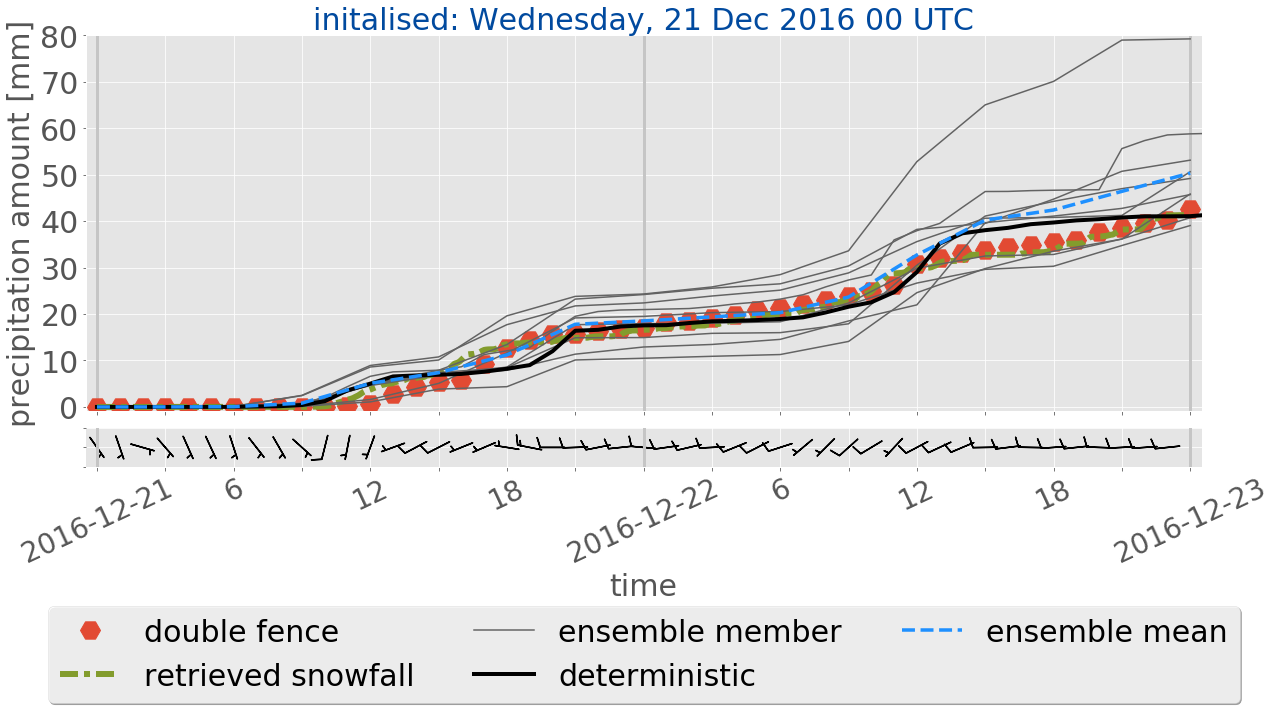
\includegraphics[trim={3.cm 2.6cm 2.cm 1.9cm},clip,width=\textwidth]{./fig_sfc_acc/acc_wind_20161221_00}
		\caption{}\label{fig:sfc_acc21}
	\end{subfigure}
	% 22/12
	\begin{subfigure}[t]{0.49\textwidth}		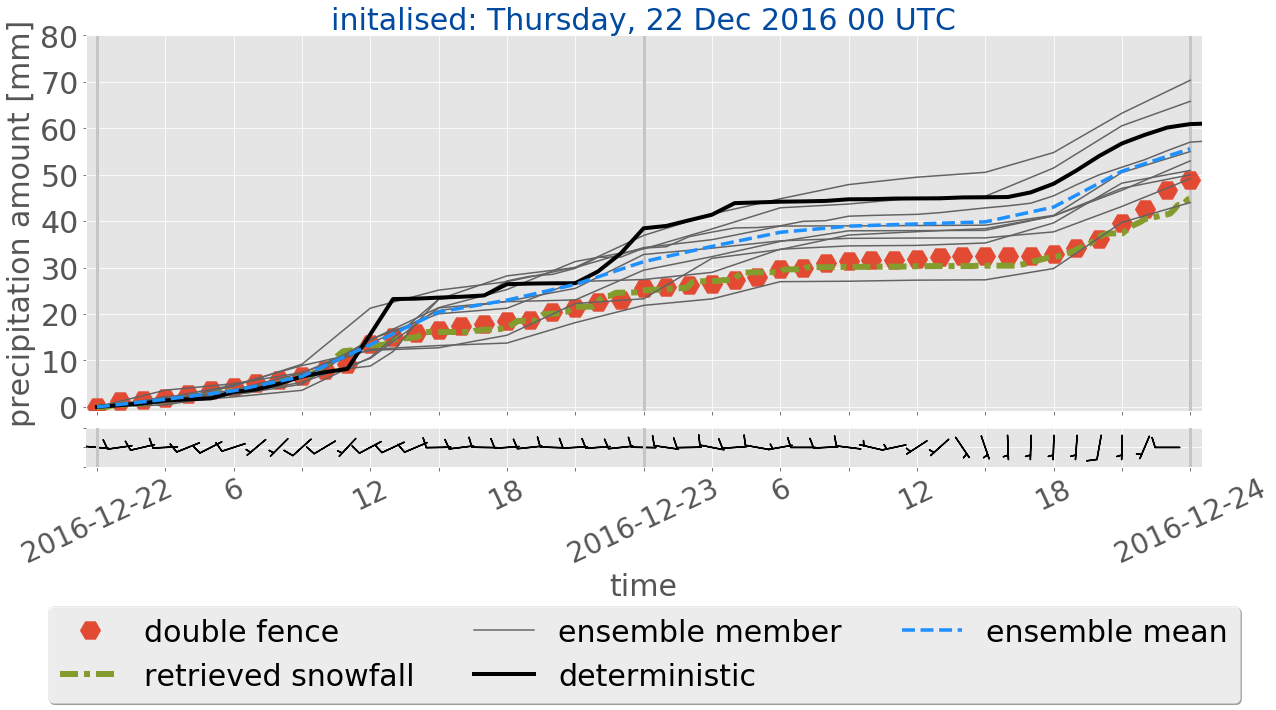
\includegraphics[trim={3.cm 2.6cm 2.cm 1.9cm},clip,width=\textwidth]{./fig_sfc_acc/acc_wind_20161222_00}
		\caption{}\label{fig:sfc_acc22}
	\end{subfigure}
	%	\end{figure}
	%   \begin{figure}\ContinuedFloat
	% 23/12
	\begin{subfigure}[t]{0.49\textwidth}	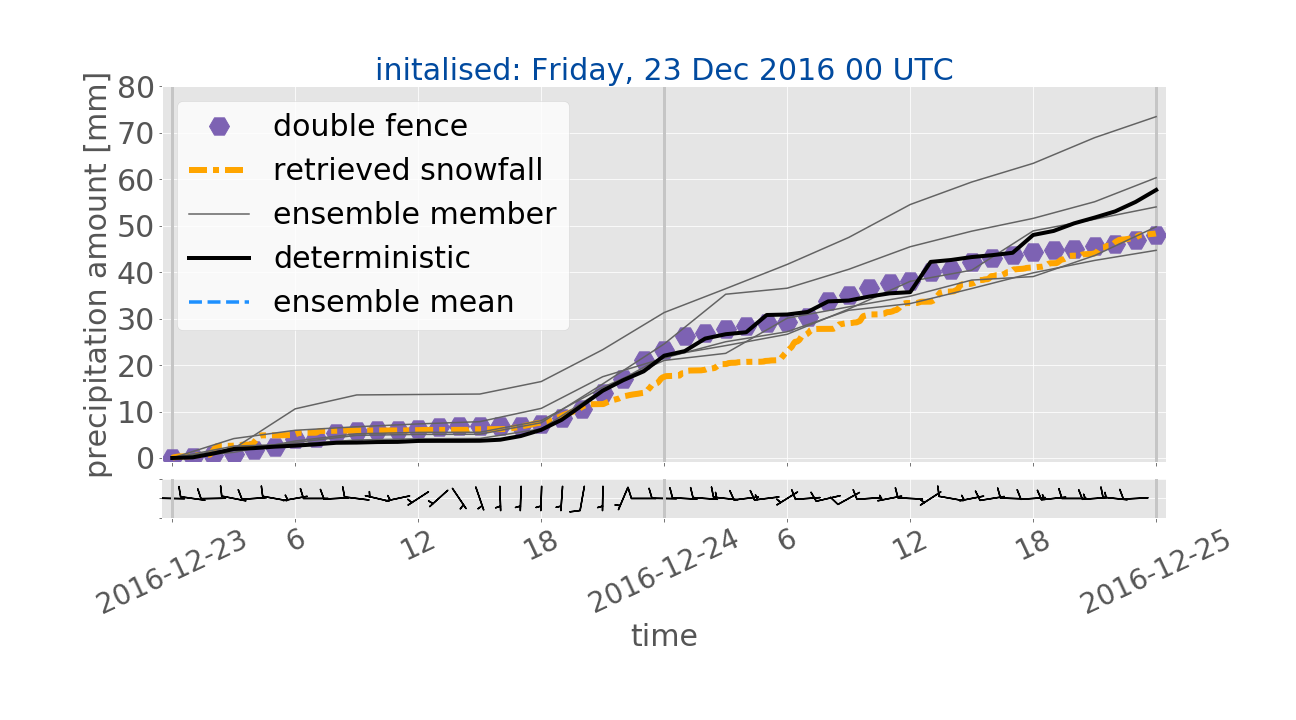
\includegraphics[trim={3.cm 2.6cm 2.cm 1.9cm},clip,width=\textwidth]{./fig_sfc_acc/acc_wind_20161223_00}
		\caption{}\label{fig:sfc_acc23}
	\end{subfigure}
	% 24/12
	\begin{subfigure}[t]{0.49\textwidth}			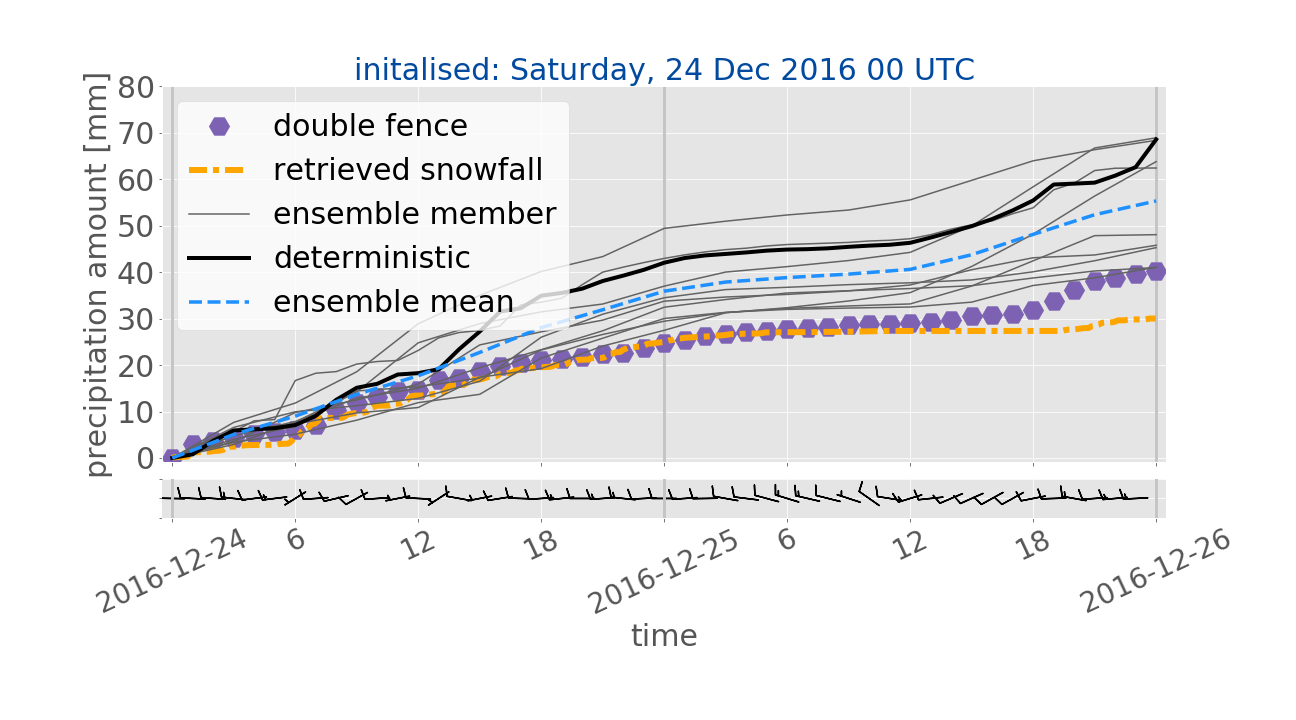
\includegraphics[trim={3.cm 2.6cm 2.cm 1.9cm},clip,width=\textwidth]{./fig_sfc_acc/acc_wind_20161224_00}
		\caption{}\label{fig:sfc_acc24}
	\end{subfigure}
	% 25/12
	\begin{subfigure}[t]{0.49\textwidth}
		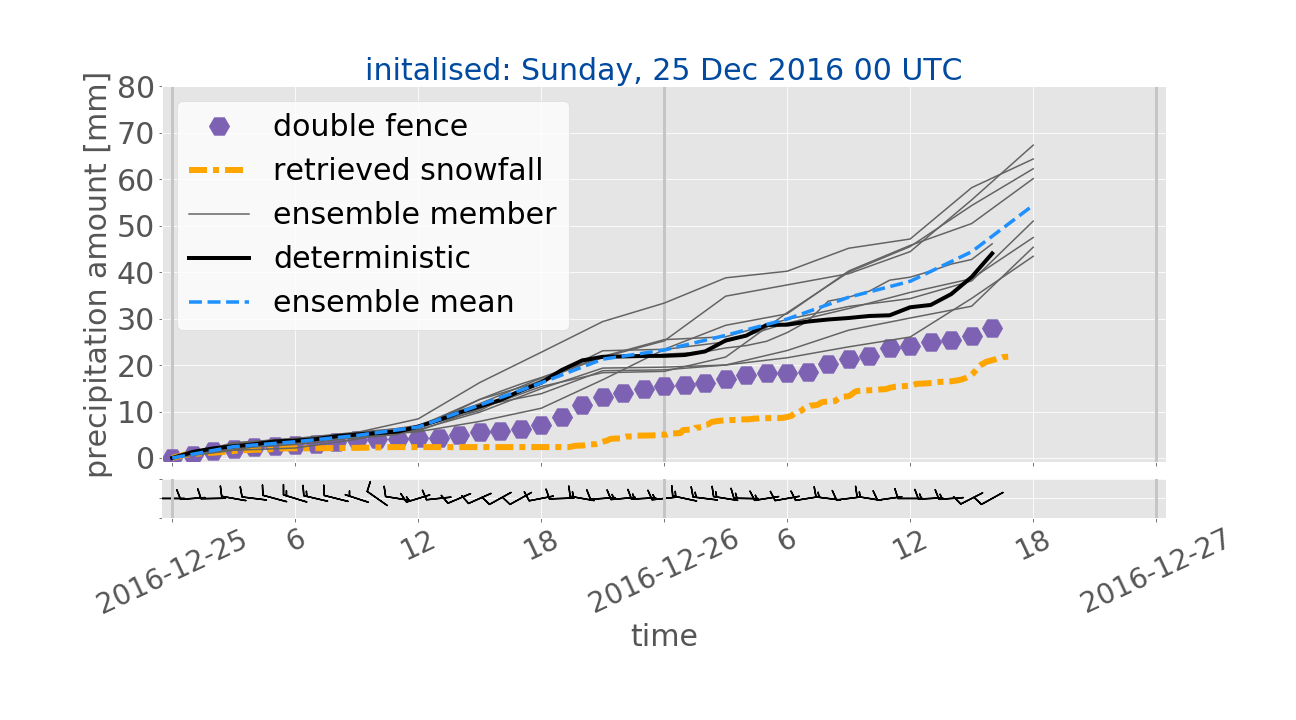
\includegraphics[trim={3.cm 2.6cm 2.cm 1.9cm},clip,width=\textwidth]{./fig_sfc_acc/acc_wind_20161225_00}
		\caption{}\label{fig:sfc_acc25}
	\end{subfigure}
	% 26/12
	\begin{subfigure}[t]{0.49\textwidth}	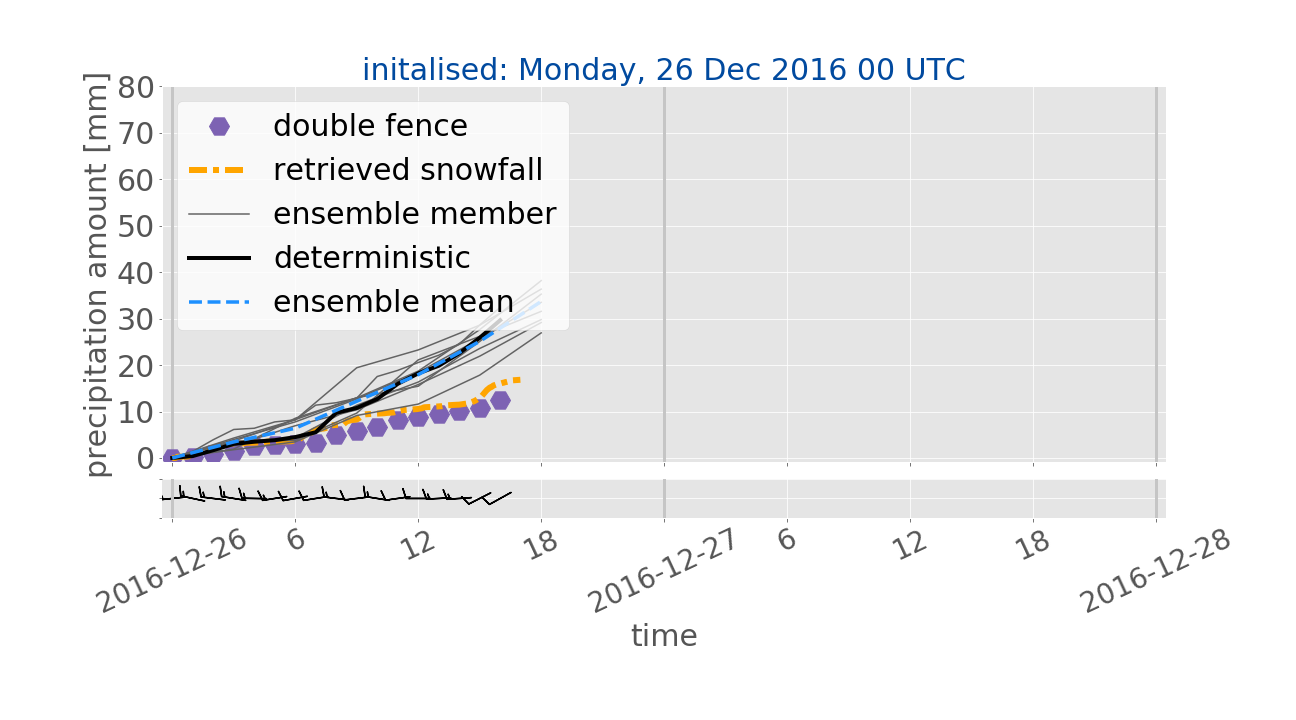
\includegraphics[trim={3.cm 2.6cm 2.cm 1.9cm},clip,width=\textwidth]{./fig_sfc_acc/acc_wind_20161226_00}
		\caption{}\label{fig:sfc_acc26}
	\end{subfigure}
	\caption{Surface snowfall accumulation. Representing the values from the double fence in purple, hexagons; optimal estimation retrieval output at snow layer height \SI{800}{\metre} in dash-dotted orange; and ensemble member deterministic forecast, initialised at 0\SI{00}{\UTC} in black and its nine perturbed ensemble members in grey. The ensemble mean of all ten members is shown in blue dashed.  Underneath are the associated last \SI{10}{\minute} average wind from the weather mast at \SI{10}{\metre} height. }\label{fig:sfc_acc}
\end{figure}


